\documentclass{beamer}

\usepackage{listings}
\usepackage[utf8]{inputenc}

 \lstdefinestyle{customc}{
  belowcaptionskip=1\baselineskip,
  breaklines=true,
  frame=L,
  xleftmargin=\parindent,
  language=C,
  showstringspaces=false,
  keywordstyle=\bfseries\color{green!40!black},
  commentstyle=\itshape\color{purple!40!black},
  tabsize=3,
  identifierstyle=\color{blue},
  stringstyle=\color{orange}
}

\lstset{escapechar=@,style=customc,numbers=left,literate={~} {$\sim$}{1}}

\setbeamerfont{framesubtitle}{size=\normalsize}
%TODO
% add frame number
% table of contents
 
%Information to be included in the title page:
\title{Software Fault Isolation using the CompCert compiler}
%\author{Alexandre Dang}
%\{Supervisor:~Frédéric Besson}
\author[\textit{Author}:~Alexandre Dang \and \textit{Supervisor}:~Frédéric Besson]
{%
	\texorpdfstring{
		\begin{columns}[t]
			\column{.45\linewidth}
				\begin{center}
				\textit{Author}: Alexandre Dang
				\end{center}
			\column{.45\linewidth}
				\begin{center}
				\textit{Supervisor}: Frédéric Besson
				\end{center}
		\end{columns}
	}
	{\textit{Auteur}: Alexandre Dang, \textit{Superviseur}: Frédéric Besson, \textit{\'Equipe}: Celtique}
}
\institute{Team Celtique}
 
\begin{document}
\frame{\titlepage}
 

%%%%%%%%%%%%%%%%%%%%  SFI  %%%%%%%%%%%%%%%%%%%%
\section{Software Fault Isolation}
\label{sec:Software Fault Isolation}



\begin{frame}{Flash vulnerable plugin}
	\begin{columns}[onlytextwidth]
		\begin{column}{0.5\textwidth}
			Do you know this logo?\\
			\vspace{5mm}
			Flash is famous for its multiple vulnerabilities\\
			$\rightarrow$~consequences on Flash\\
			$\rightarrow$~but ALSO endangers your browser
		\end{column}
		\begin{column}{0.5\textwidth}
			\begin{figure}
				\centering
				
\includegraphics[width=0.7\textwidth]{images/flash.jpg}
			\end{figure}
		\end{column}
	\end{columns}
\end{frame}


\begin{frame}{Goals of Software Fault Isolation (SFI)~\cite{Wahbe:1993:ESF:173668.168635}}
	\begin{itemize}\itemsep20pt
		\item SFI aims to allow a protected program to execute dangerous modules in its own memory space without dangers. 
		\item SFI confines the execution of the dangerous modules in a reserved memory space called sandbox
	\end{itemize}
\end{frame}

\begin{frame}[c]{Goals of SFI}
\begin{figure}
\centering
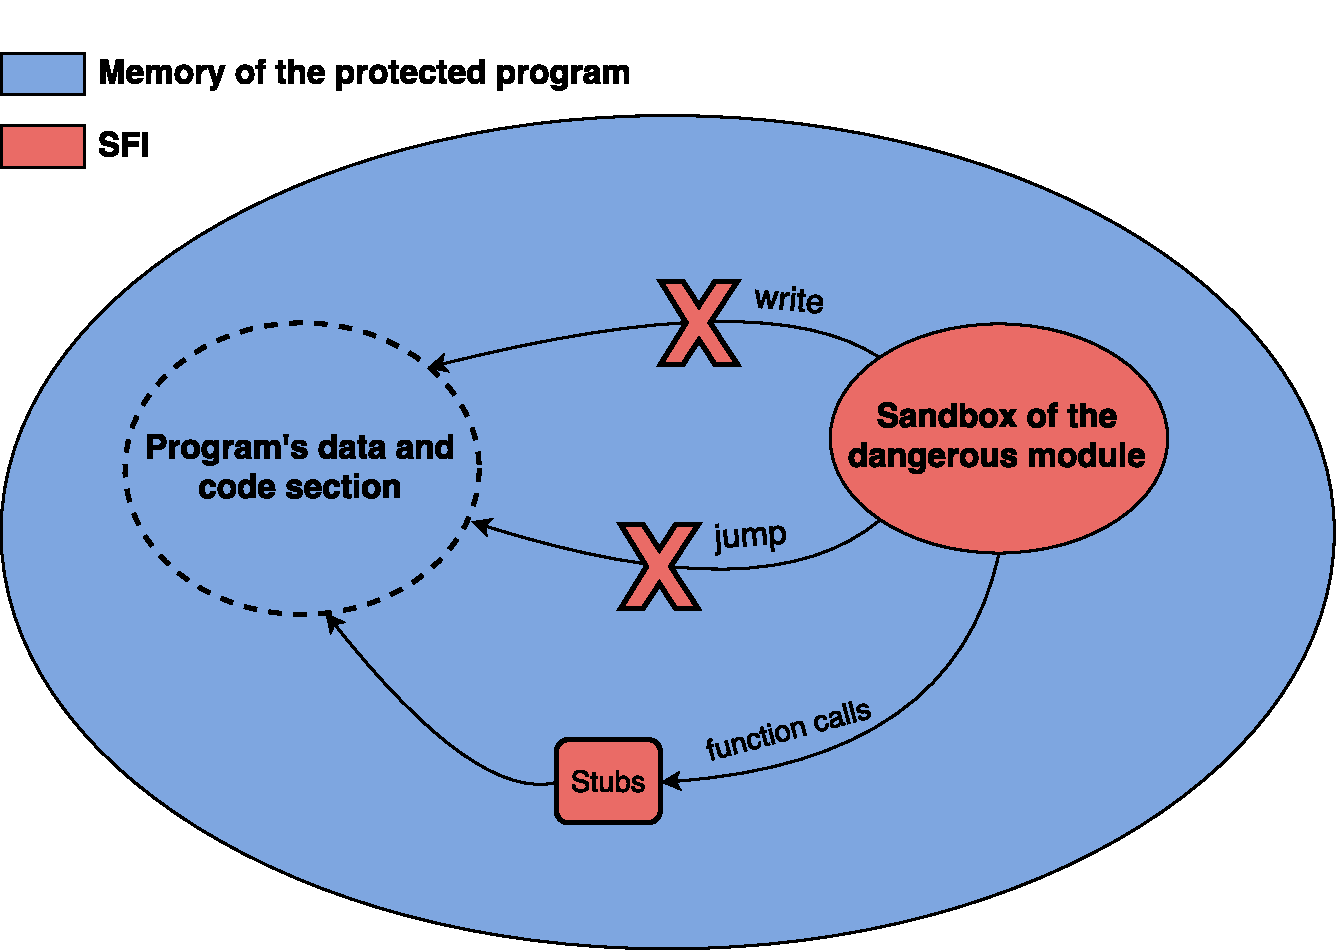
\includegraphics[width=1\textwidth]{images/sfi_principle.pdf}
\end{figure}

\end{frame}

\begin{frame}{Overview of SFI} %code gen + verifier
	SFI chain is composed of two elements:
		\begin{itemize}
			\item the \textbf{generator} transforms the assembly code of the dangerous modules in order to confine the modules in their sandbox
			\item the \textbf{verifier} checks that the SFI transformations are present and valid before loading the code in memory
		\end{itemize}
		\vspace{5mm}
		\begin{columns}
			\column{\dimexpr\paperwidth-10pt}
			\begin{center}
			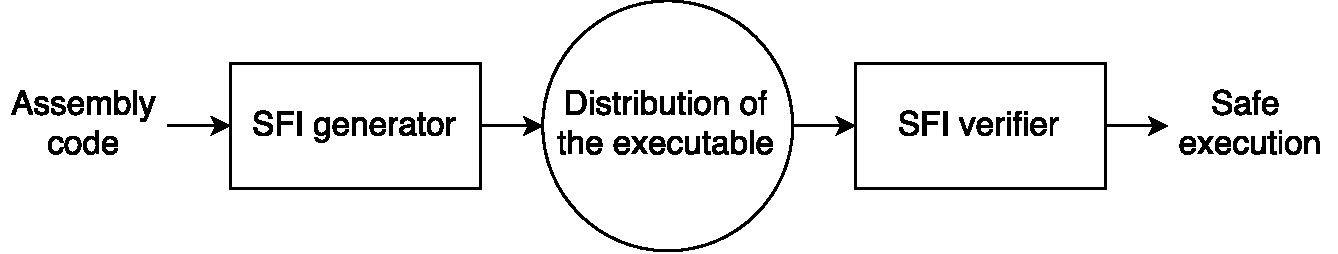
\includegraphics[width=0.95\paperwidth]{images/sfi_chain.pdf}
			\end{center}
		\end{columns}
\end{frame}

\begin{frame}[c]{Problematics of SFI}
We want to prevent attackers from using vulnerable modules to compromise our system
	\begin{itemize}
		\item SFI gives us a way to face such issue
		\item However SFI is currently lacking against Returned Oriented Programing attacks (ROP)
		\item ROP attacks focus function return addresses to execute malicious code they injected
	\end{itemize}
	
\end{frame}

%%%%%%%%%%%%%%%%%%%%  ROP  %%%%%%%%%%%%%%%%%%%%
% Faire un scnario plutôt avec un mdp revele
\section{Return Oriented Programing attacks}
\label{sec:Return Oriented Programing attacks}

\defverbatim[colored]\Buffer{%
\begin{lstlisting}[tabsize=2,frame=single]
void reset_password() {
	... reset password ...			//Sensitive code
}

void foo(char* input){
	char buf[1];
	... code ...
	strcpy(buf, input);					//Vulnerability
	... code ...
}
\end{lstlisting}}

\begin{frame}{ROP attack example (1/2)}
	\Buffer
\end{frame}

\begin{frame}[c]{ROP attack example (2/2)}
	\center
	\vspace{-10mm}
	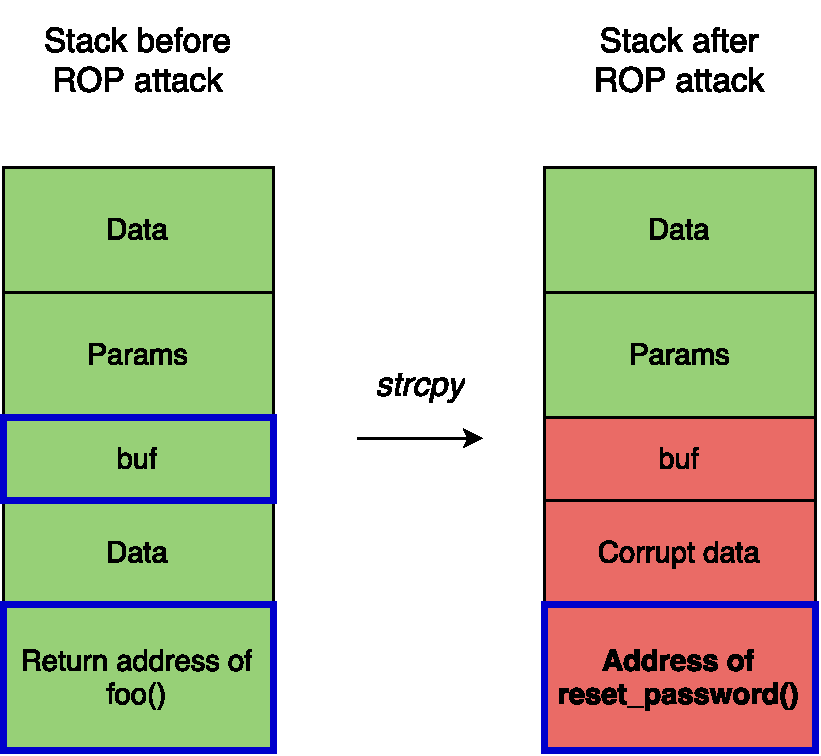
\includegraphics[height=0.7\textheight]{images/bof_stack.pdf}
\end{frame}

\begin{frame}[c]{Modern ROP attacks}
	\begin{itemize}
		\item ROP attacks are a common kind of attack in the industry
		\item Modern ROP attacks are much more complicated~\cite{BRSS08}
	\end{itemize}
	\hfill \break
	\begin{center}
		\textit{``Skype URI handling\\ routine contains a buffer overflow''}, 2005\footnotemark \\
	\end{center}
	\vspace{4mm}
	\textit{``Apple Mail buffer \\overflow vulnerability``}, 2006\\
	\begin{flushright}
		\textit{''glibc vulnerable to stack buffer \\overflow in DNS resolver``}, 2016
	\end{flushright}

	\footnotetext{From CERT vulnerability database}
\end{frame}




%%%%%%%%%%%%%%%%%%%%  Overview  %%%%%%%%%%%%%%%%%%%%
%Contributions
%Table des matières
%Enoncer les problematiques (localisation des addresses de retour
\section{Overview of our approach}
\label{sec:Overview of our approach}

%\begin{frame}[c]{Goals of our approach}
%	We want to have a way to protect return addresses at runtime.
%	\begin{itemize}
%		\item Modifications of the memory layout in order to have an easy way to know return addresses location
%		\item Code transformations which add runtime checks on the dangerous instruction in order to forbid any illegal \texttt{write} on the return addresses locations
%	\end{itemize}
%\end{frame}

\begin{frame}[c]{Contributions}
\begin{itemize}\itemsep20pt
		\item An approach protecting return addresses against ROP attacks
		\item An implementation of our approach with the compiler CompCert for the x86-32 architecture
	\end{itemize}
\end{frame}


\begin{frame}[c]{Problematic}
	We want to add additional checks at runtime to protect the return addresses. \\
	\begin{center}
		{\Large How do we know the return addresses locations in the memory?}	
		\break
		\break
		\visible<2>{\textcolor{red}{$\Rightarrow$~Modify the memory structure to have an easy way to distinguish return addresses locations}}
	\end{center}
\end{frame}

\begin{frame}[c]{Presentation of our approach}
	\begin{enumerate}\itemsep16pt
		\item Presentation of the stack
		\item Transformation of the stack structure
		\item Insertion of runtime checks in the protected code
		\item Evaluation of the approach
	\end{enumerate}
\end{frame}


\begin{frame}[c]{Stack structure}
	\begin{columns}
		\begin{column}{0.55\textwidth}
			\begin{itemize}
				\item Programs memory is separated into multiple area like the heap, the stack or the code section
				\item Return addresses are solely located in the stack
				\item The stack is composed of piled up frames each related to a function being executed
				\item Frames store data of their respective function
			\end{itemize}
		\end{column}
		\begin{column}{0.45\textwidth}
			\begin{figure}
			\centering
			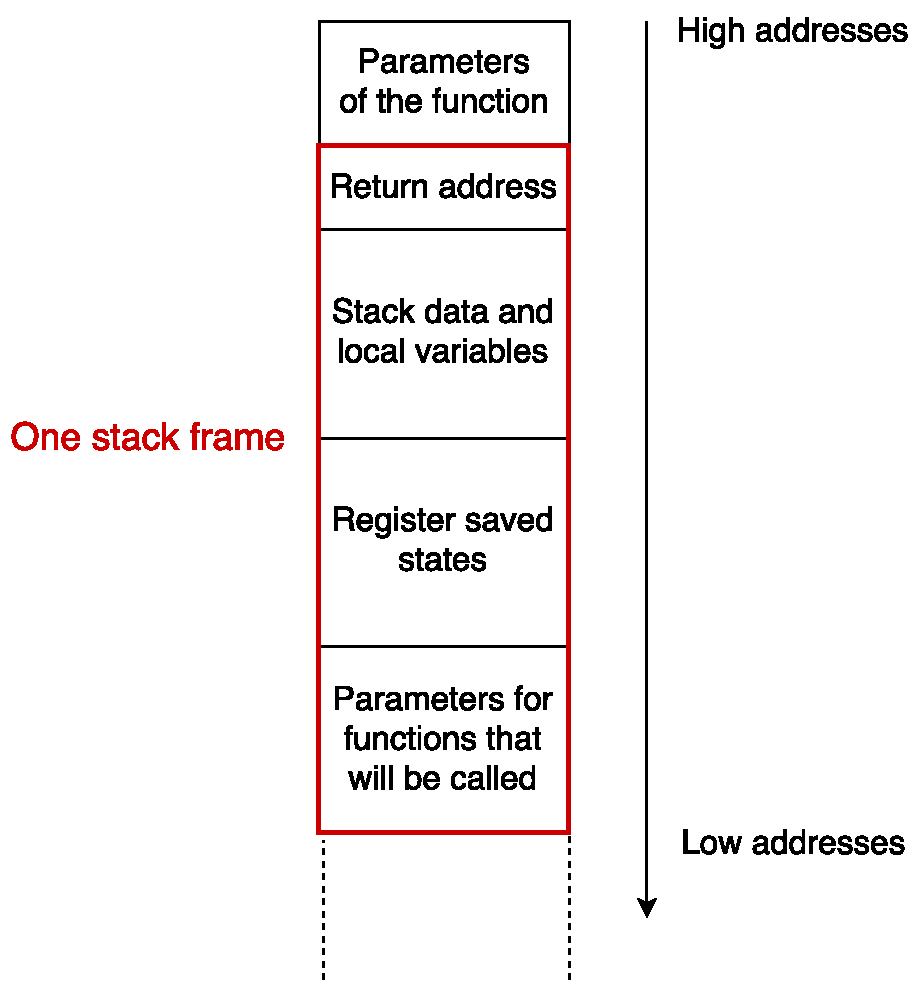
\includegraphics[height=0.75\textheight]{images/stack_layout.pdf}
			\end{figure}
		\end{column}
	\end{columns}
\end{frame}

\begin{frame}[c]{Stack transformation objective}
	\begin{itemize}\itemsep16pt
		\item We want a stack structure with a property on the return addresses locations
		\item Every return addresses location $a$ verifies the equality \underline{$a~mod~n=0$}
		\item The transformation is composed of two steps:
			\begin{enumerate}
				\item Constant frames size
				\item Stack alignment
			\end{enumerate}
	\end{itemize}
\end{frame}

%Faire un graphe evolutif
\begin{frame}[c]{Stack transformation (1/6)}{Find the biggest frames size}
	\begin{center}
		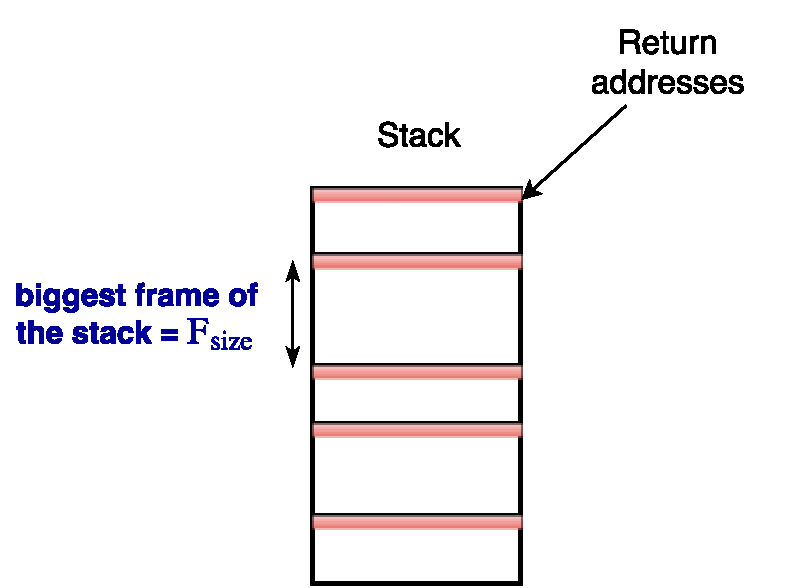
\includegraphics[height=0.6\textheight]{images/stack_transfo_0.pdf}
	\end{center}
\end{frame}
%height=0.85\textheight
\begin{frame}[c]{Stack transformation (2/6)}{Calculate the new frames size}
	\begin{center}
		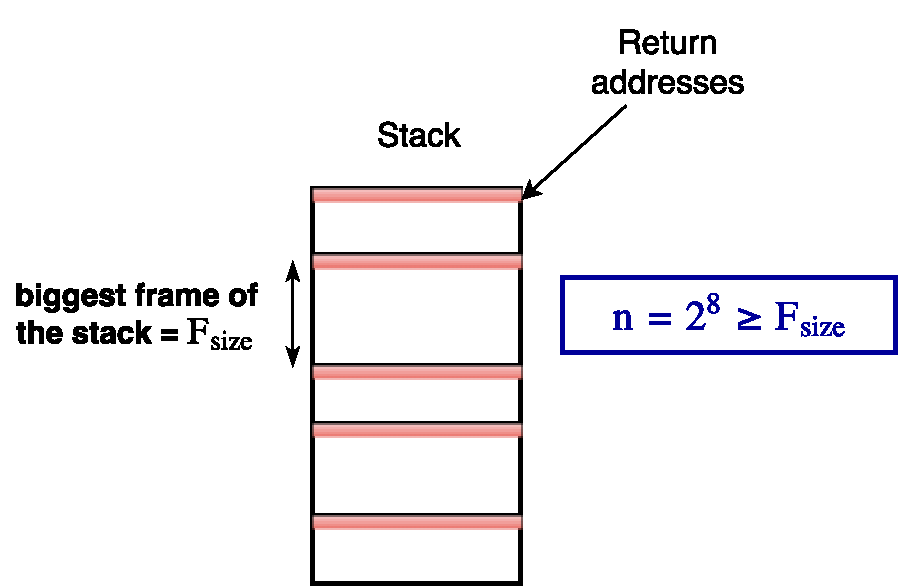
\includegraphics[height=0.6\textheight]{images/stack_transfo_1.pdf}
	\end{center}
\end{frame}
\begin{frame}[c]{Stack transformation (3/6)}{Fix the size of the frames}
	\begin{center}
		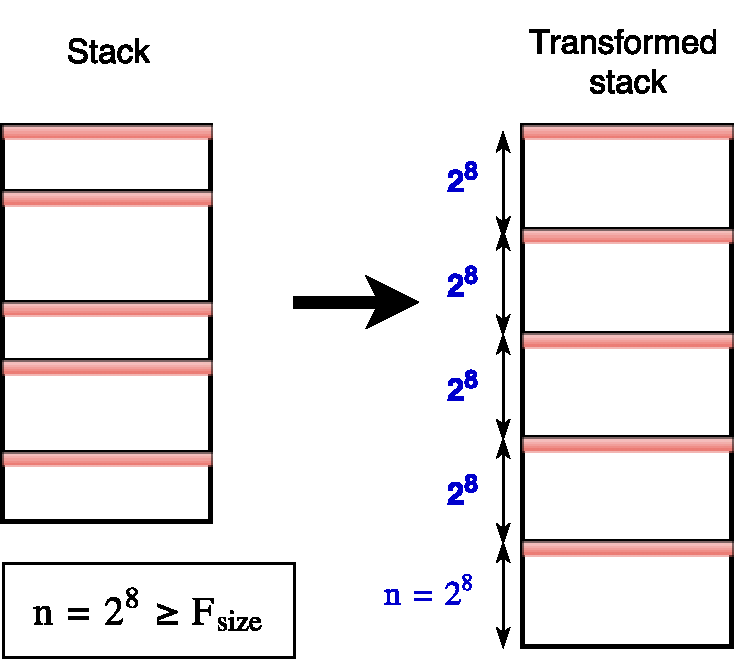
\includegraphics[height=0.7\textheight]{images/stack_transfo_2.pdf}
	\end{center}
\end{frame}
\begin{frame}[c]{Stack transformation (4/6)}{Return addresses locations}
	\begin{center}
   		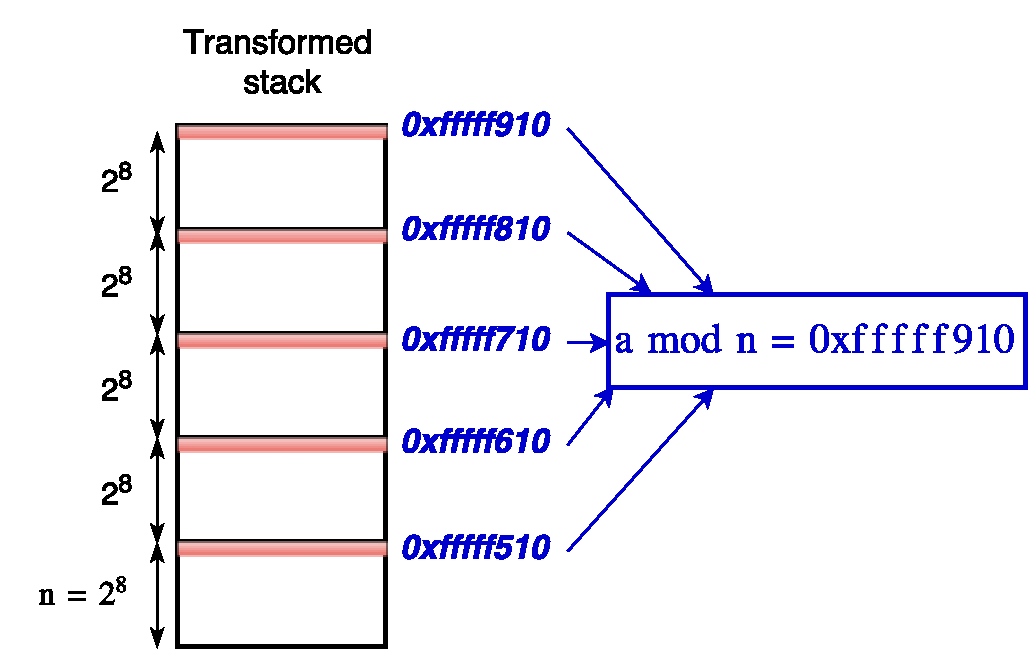
\includegraphics[width=0.9\textwidth]{images/stack_transfo_3.pdf}
	\end{center}
\end{frame}
\begin{frame}[c]{Stack transformation (5/6)}{Insertion of a new artificial main}
	\begin{center}
		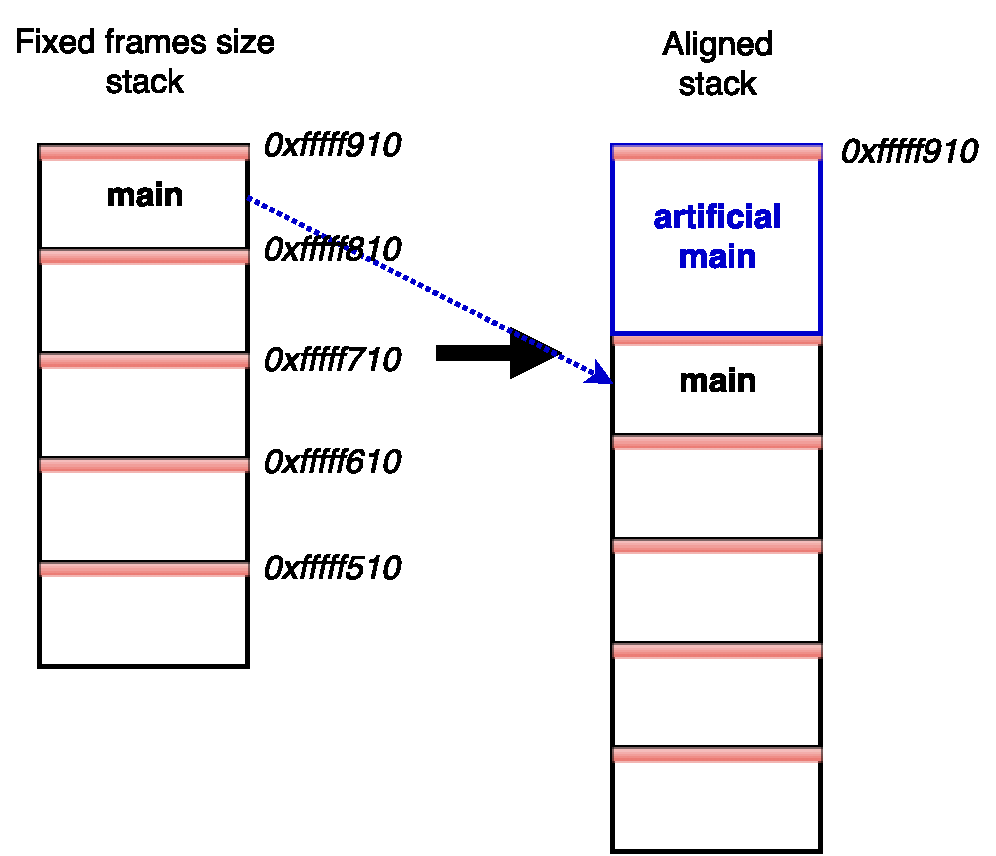
\includegraphics[height=0.75\textheight]{images/stack_transfo_4.pdf}
	\end{center}
\end{frame}
\begin{frame}[c]{Stack transformation (6/6)}{Return addresses locations}
	\begin{center}
   		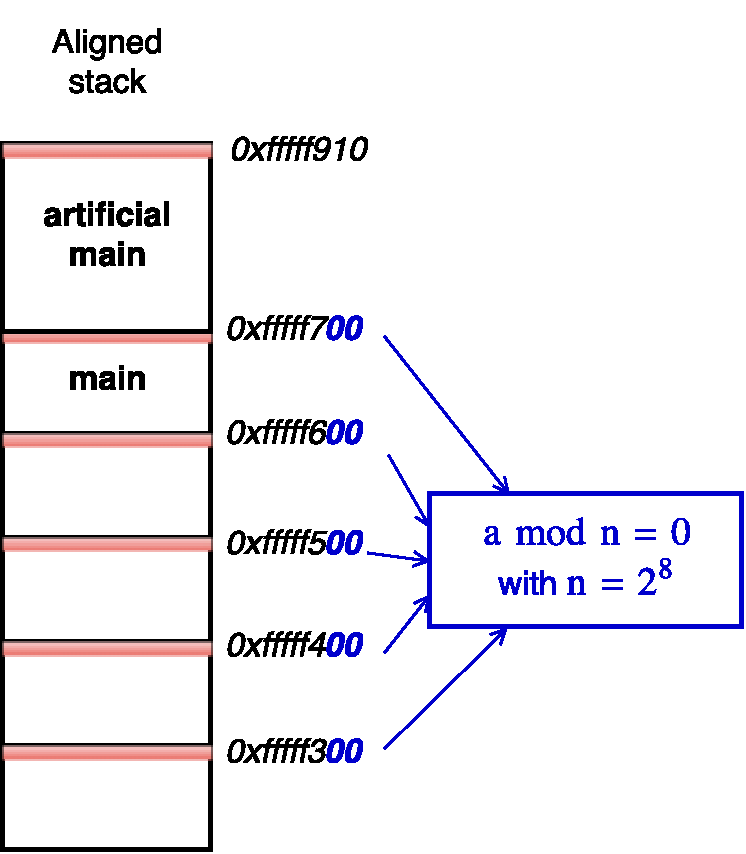
\includegraphics[height=0.75\textheight]{images/stack_transfo_5.pdf}
	\end{center}
\end{frame}

%begin{frame}[c]{Transformations of the stack layout}
%   All the return addresses locations $a$ verify the equality $a~mod~n=0$, with $n$ a constant offset between the return addresses locations.
%   \begin{enumerate}
%   	\item Set a constant offset $n$ between all the return addresses
%   	\item Align the stack
%   \end{enumerate}
%end{frame}
%
%begin{frame}[c]{Constant offset $n$ between return addresses (1/2)}
%   Constant offset $n$ between return addresses locations
%   \begin{itemize}
%   	\item Fix frames size to $n$
%   	\item Pick $n$ as the biggest frame size of the previous stack
%   	\item Pick $n$ as a power of two
%   \end{itemize}
%   With this we have $a~mod~n=c$, with $c$ the location of the first return address in the stack
%end{frame}
%
%begin{frame}[c]{Constant offset $n$ between return addresses (2/2)}
%   \begin{figure}
%   \centering
%   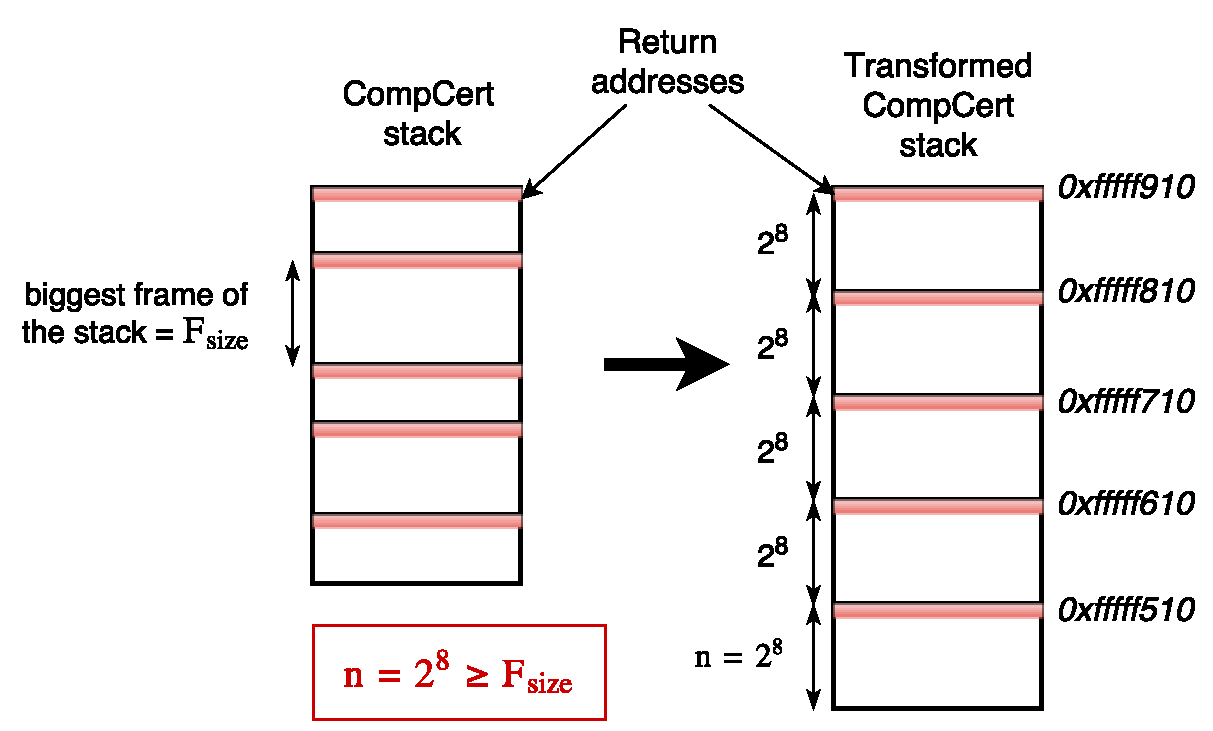
\includegraphics[width=\textwidth]{images/stack_transform.pdf}
%   \end{figure}
%end{frame}
%
%begin{frame}[c]{Stack alignment (1/2)}
%   We currently have the equality $a~mod~n=c$ but we want $a~mod~n=0$ with $a$ any return address locations  and $c$ the first return address location in the stack.
%   \begin{itemize}
%   	\item introduce an artificial function at the beginning of the program
%   	\item the function align the stack as we wanted
%   	\item the function then calls the \textit{main} of the program
%   \end{itemize}
%end{frame}
%
%begin{frame}[c]{Stack alignment (2/2)}
%   \begin{figure}
%   \centering
%   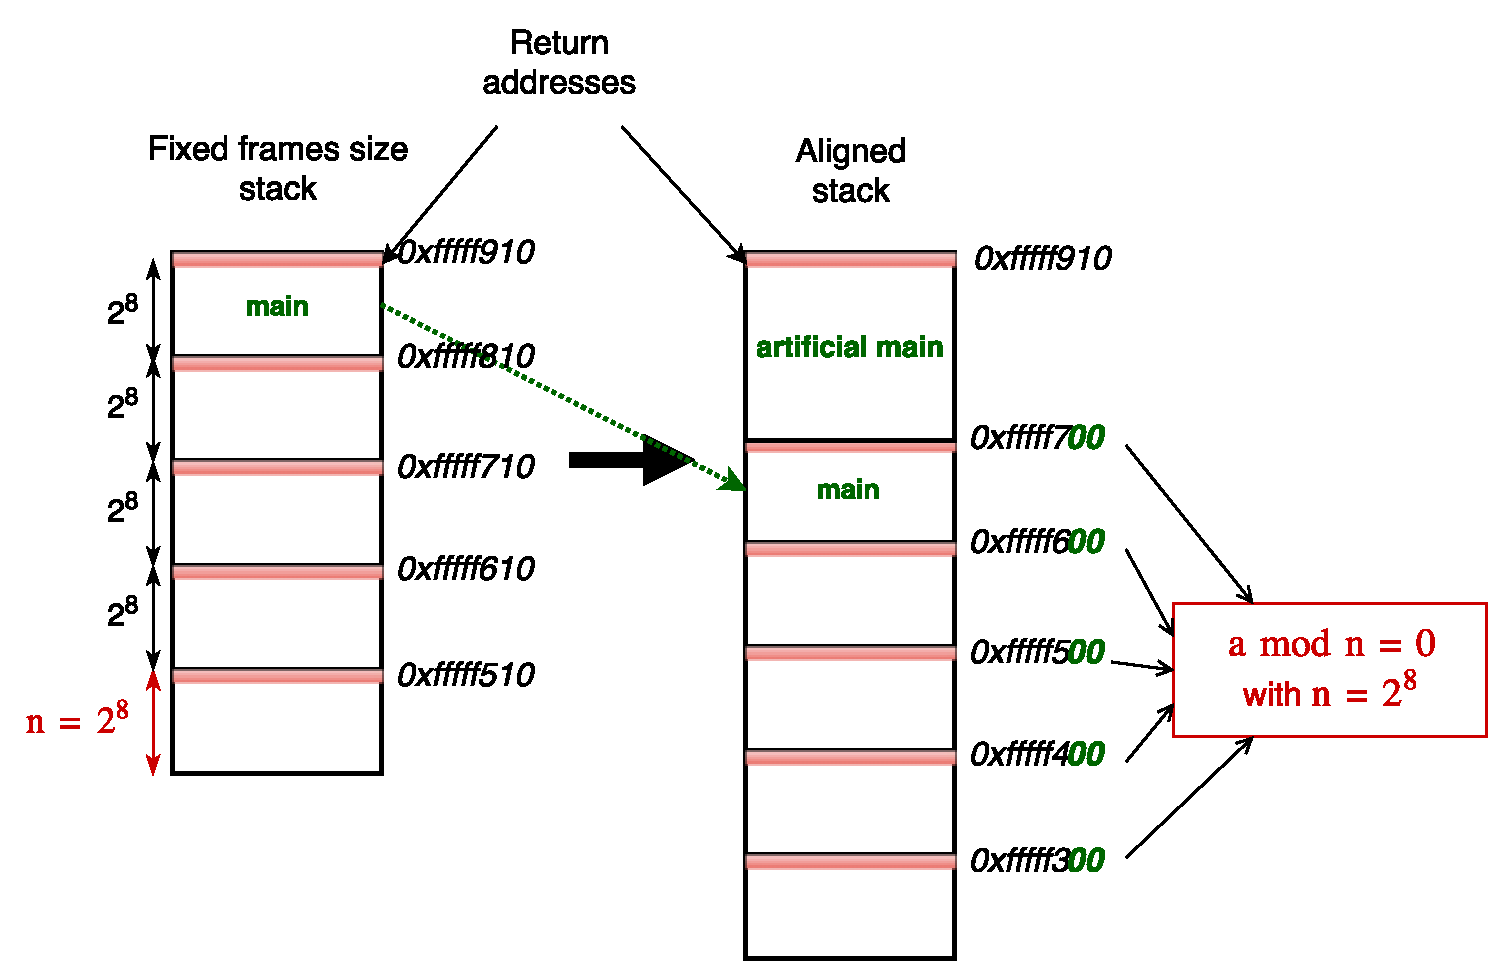
\includegraphics[width=\textwidth]{images/stack_align.pdf}
%   \end{figure}
%end{frame}

\begin{frame}[c]{Code transformation}
	\begin{itemize}\itemsep20pt
		\item We have now an easy way to differentiate return addresses locations with $a~mod~n=0$
		\item We need to insert additional runtime check to protect these locations from being overwritten illegally
		\item Thus we transform the code adequately during the compilation phase
	\end{itemize}
\end{frame}

\begin{frame}[c]{Runtime check}
	\vspace{-8mm}
	\hspace{30mm}
   	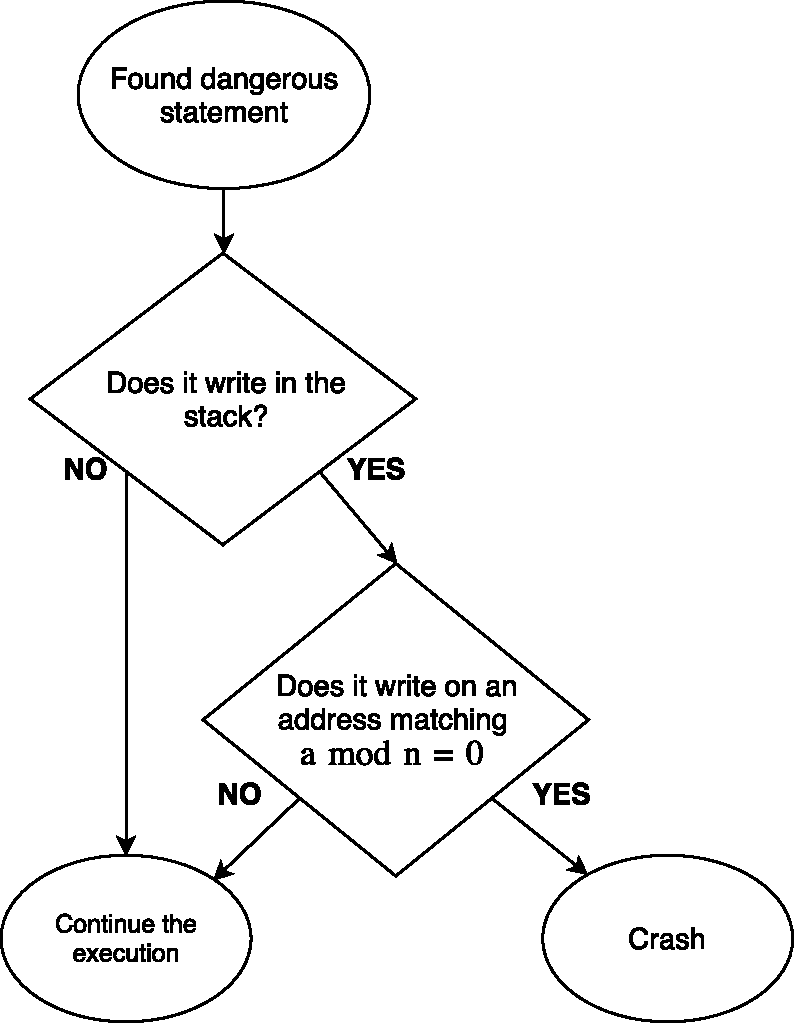
\includegraphics[height=0.95\textheight]{images/runtime_check.pdf}
\end{frame}

\begin{frame}[c]{Branchless check}
	\hspace{30mm}
	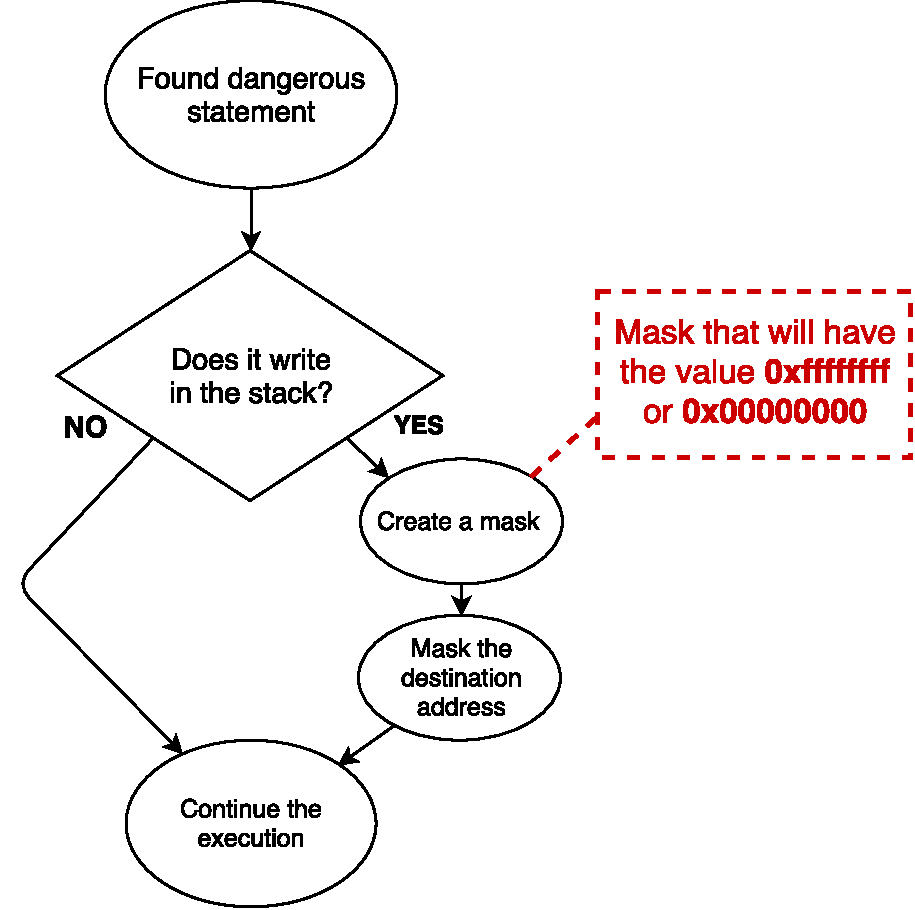
\includegraphics[height=0.8\textheight]{images/branchless_check.pdf}
\end{frame}
%\defverbatim[colored]\Check{%
%\begin{lstlisting}[tabsize=2,frame=single]
%if (targeted_address > 0xff000000) {
%	temp_var = targeted_address & (n-1);
%	if (temp_var < 3) {
%		Error behaviour
%	} 
%}
%*targeted_address = value;
%Continue execution...
%\end{lstlisting}}
%
%\begin{frame}[fragile]{Injection of runtime checks}
%	\begin{enumerate}
%		\item Check if the address is part of the stack
%		\item Check if the address verifies $a~mod~n=0$
%	\end{enumerate}
%	\hfill \break
%	\Check
%\end{frame}
%\defverbatim[colored]\Branchless{%
%\begin{lstlisting}[tabsize=2,frame=single]
%if (targeted_address > 0xff000000) {
%		temp_var = targeted_address & (n-1);
%		temp_var = temp_var - 3;
%		temp_var = temp_var >> 31;
%		temp_var = ~temp_var;
%		targeted_address = temp_var & targeted_address;
%}
%*targeted_address = value;
%Continue execution...
%\end{lstlisting}}
%
%%Diagramme
%\begin{frame}{Branchless runtime checks}
%	In certain cases  branchless code shows much better performance
%	\Branchless
%\end{frame}
%

\begin{frame}[c]{Implementation environment}{CompCert the certified compiler~\cite{Leroy:2009:FVR:1538788.1538814}}
	\begin{itemize}
		\item CompCert has been proven with the proof assistant Coq
		\item CompCert has performance similar to \texttt{gcc -O1}
	\end{itemize}
	\hfill \break
	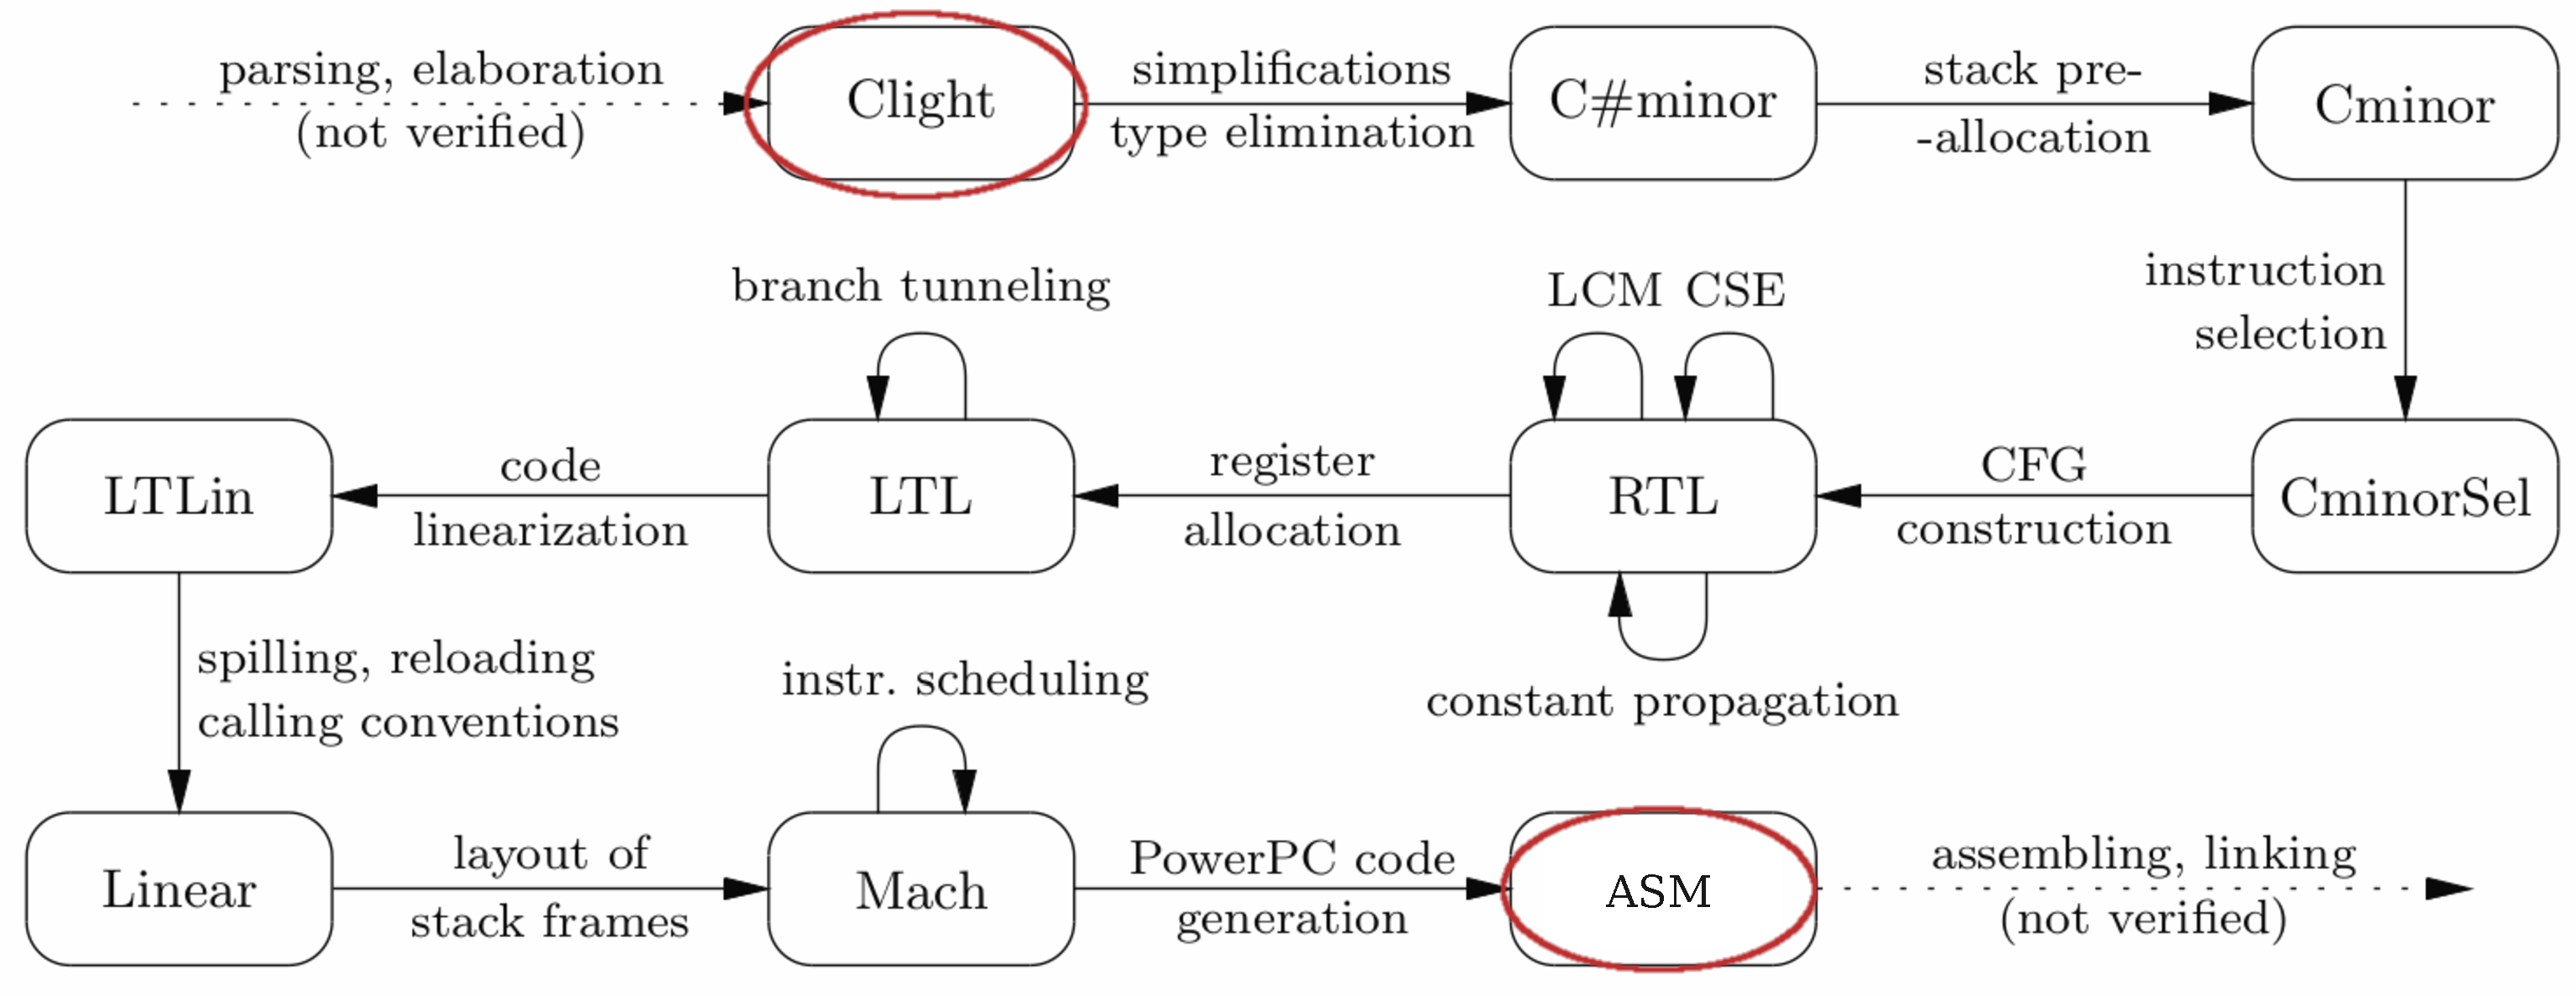
\includegraphics[width=\textwidth]{images/compcert_pass.pdf}
\end{frame}

\begin{frame}[fragile]{Necessary requirements}
	\begin{itemize}
		\item No modifications of the stack (inline assembly)
			\begin{lstlisting}[tabsize=2,frame=single,linewidth=7cm]
			int foo(int a) {
				asm(``\$sub 50, \%esp'');
				printf("Hello world!");
			}
			\end{lstlisting}
		\item No function pointers to protect our runtime checks
		\item Need to recompile external libraries with the same frames size
	\end{itemize}
\end{frame}

%%%%%%%%%%%%%%%%%%%%  Evaluation  %%%%%%%%%%%%%%%%%%%%
\section{Evaluation}
\label{sec:Implementation}

%Changer couleurs et mettre plus de graphes
\begin{frame}[c]{Evaluation of performance }
	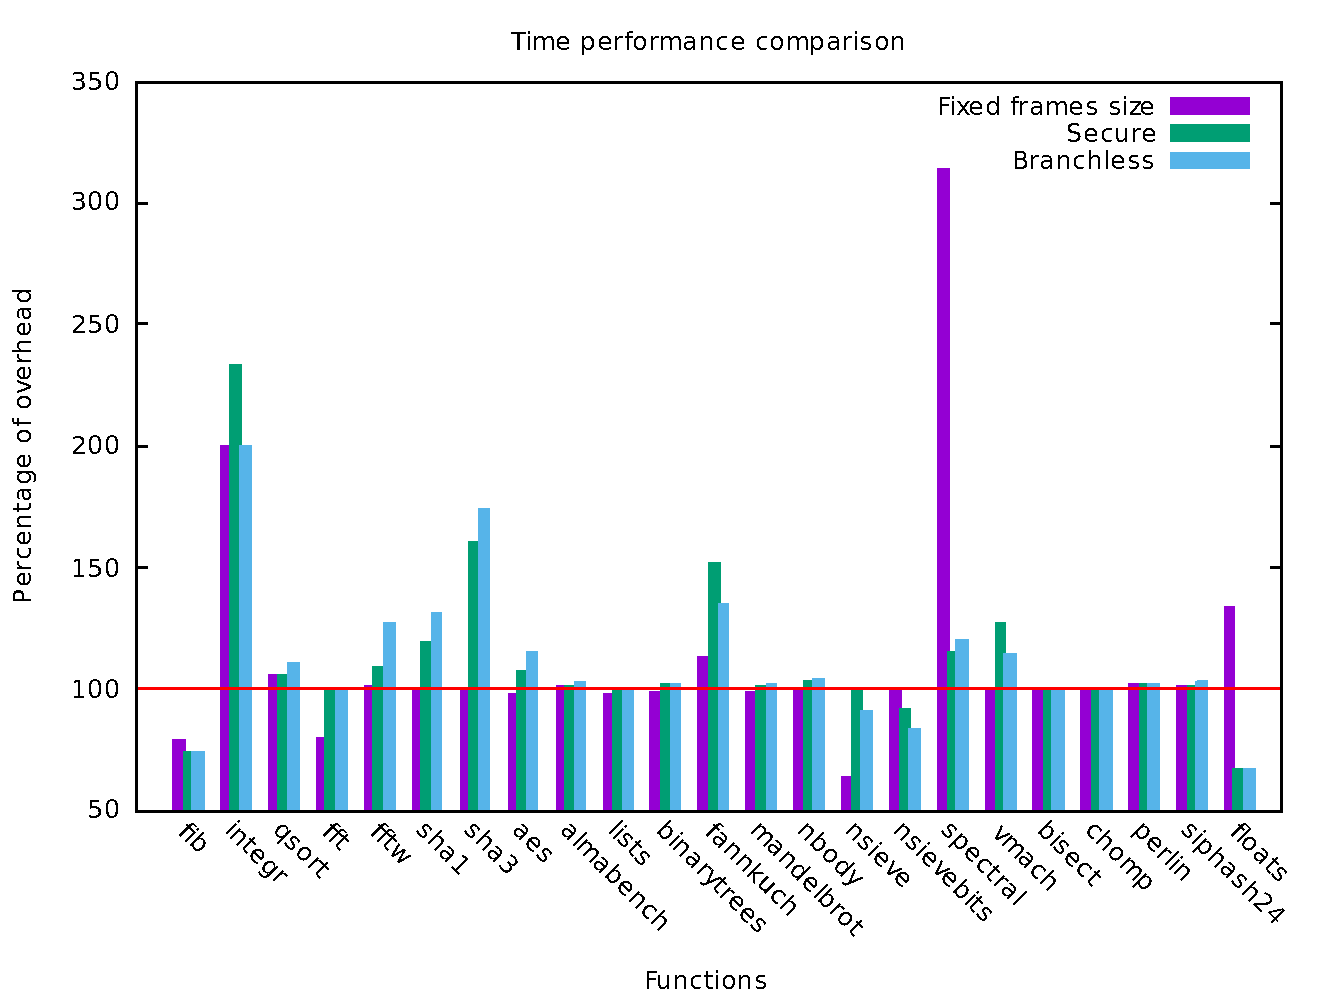
\includegraphics[width=\textwidth]{images/time_percentage_graph.pdf}
\end{frame}

\begin{frame}[c]{Evaluation of performance }
	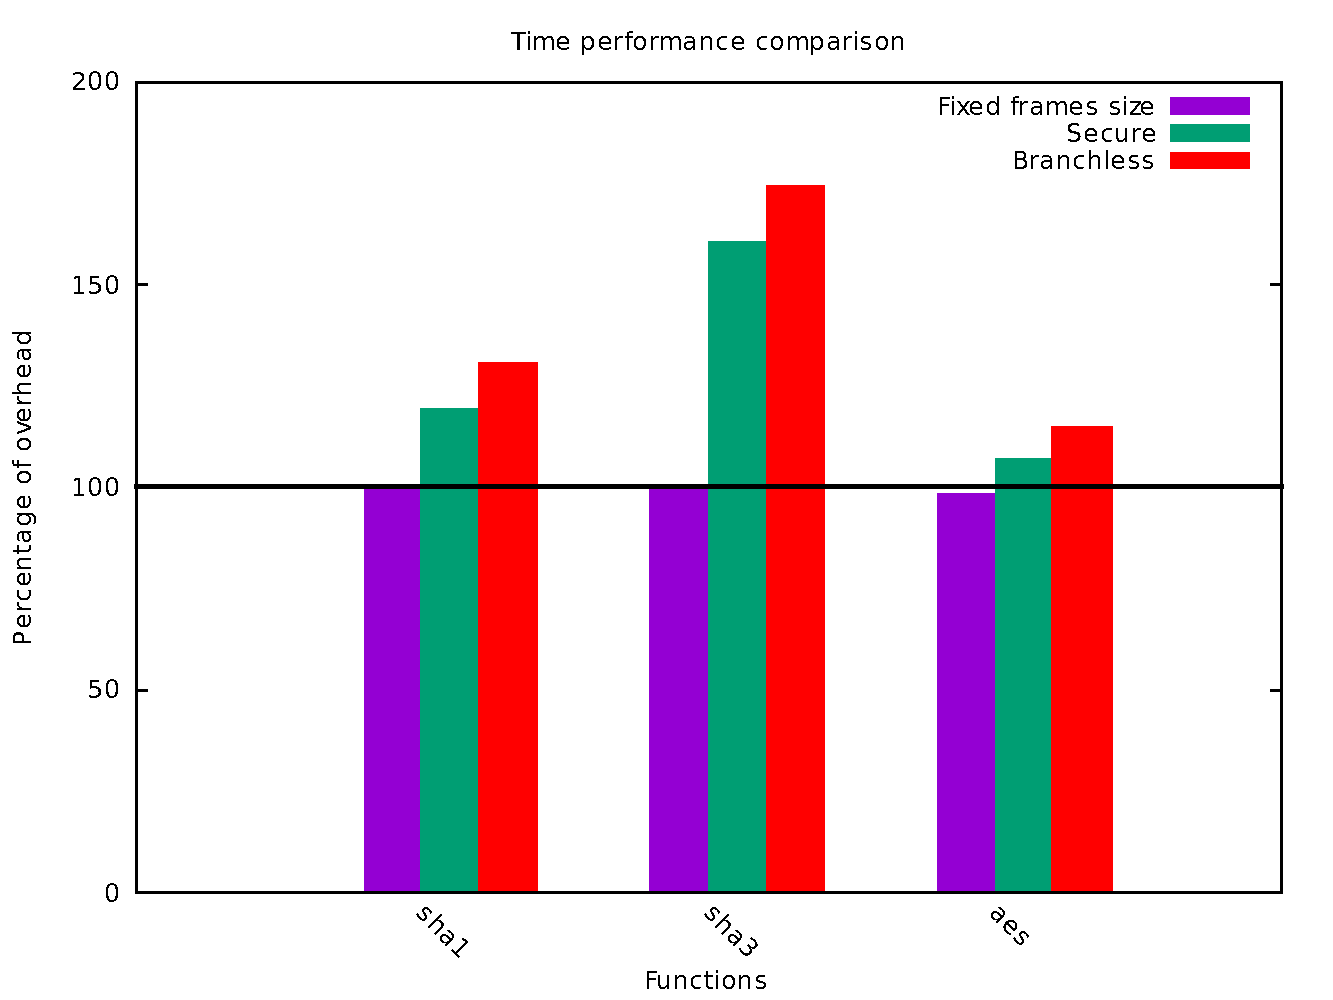
\includegraphics[width=\textwidth]{images/percentage_focus.pdf}
\end{frame}


\begin{frame}[c]{Conclusion}
	\underline{Prospectives}
	\begin{itemize}
		\item Test our implementation against more complicated ROP attacks
		\item Reduce the number of runtime checks with static analysis~\cite{Zeng:2011:CCI:2046707.2046713}
		\item Improve the performance of the runtime checks with a super-optimizer
		\item See the impact of our approach on memory consumption
	\end{itemize}
\end{frame}

 
\nocite{Leroy:2009:FVR:1538788.1538814}
\nocite{Sehr:2010:ASF:1929820.1929822}
\nocite{Wahbe:1993:ESF:173668.168635}
\nocite{Zeng:2011:CCI:2046707.2046713}

\begin{frame}[noframenumbering]{References}
	\scriptsize
	\setbeamertemplate{bibliography item}{\insertbiblabel}
	\bibliographystyle{plain}
    \bibliography{ref}
\end{frame}

\end{document}


